\documentclass{beamer}

\usepackage{graphicx}
\usepackage{minted}

% === customization.sty ===
\usetheme{Copenhagen}

\addtobeamertemplate{navigation symbols}{}{%
    \usebeamerfont{footline}%
    \usebeamercolor[fg]{footline}%
    \hspace{1em}%
    \insertframenumber/\inserttotalframenumber
}
% from https://tex.stackexchange.com/questions/137022/how-to-insert-page-number-in-beamer-navigation-symbols

%\AtBeginSection[]
%{
  %\begin{frame}
    %\frametitle{Table of Contents}
    %\tableofcontents[currentsection]
  %\end{frame}
%}
% from https://www.overleaf.com/learn/latex/Beamer#Customizing_your_presentation
% === end customization.sty ===

\begin{document}

\title{Haskell for Web Apps: A Human Task Scheduler}
\subtitle{Backend and Frontend in One Reliable Language}
\author{Bisma Rohpanca Joyosumarto}
%\date{Tuesday, 10 December 2024}
\date{December 2024}

\frame{\titlepage}

\begin{frame}{About Me}
    \begin{tabular}{cl}
        \begin{tabular}{c}
            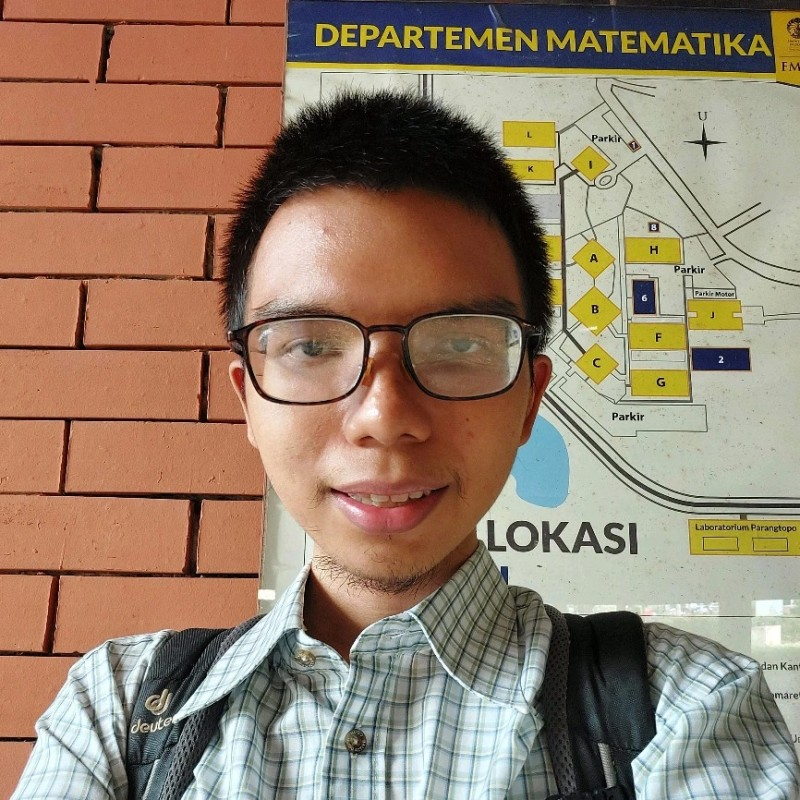
\includegraphics[height=4cm, width=4cm]{profile_pic.jpeg}
        \end{tabular}
        &
        \begin{tabular}{l}
            \parbox{0.5\linewidth}{%  change the parbox width as appropiate
            \begin{itemize}
                \item Undergraduate Final Year Mathematics Student at University of Indonesia
                \item Interests:
                \begin{itemize}
                    \item Reliable and verified systems
                    \item Building technology to help make people's lives easier
                    \item Mathematics and its applications
                \end{itemize}
            \end{itemize}
            }
        \end{tabular}
    \end{tabular}
    % ref: https://tex.stackexchange.com/questions/165475/figure-next-to-text-in-beamer
\end{frame}

\begin{frame}{Table of Contents}
    \tableofcontents
\end{frame}

\section{The Web App: A Human Task Scheduler}

\begin{frame}{The Need for A Task Scheduler}
    \begin{itemize}
        \item 
    \end{itemize}
\end{frame}

\begin{frame}{The Idea: Human Task Scheduler}
    \begin{itemize}
        \item 
    \end{itemize}
\end{frame}

\section{The Technology: Haskell}

\begin{frame}{Haskell for Backend}
    
\end{frame}

\begin{frame}{Haskell for Frontend}
    
\end{frame}

\section{Key Takeaways}

\begin{frame}{Key Takeaways}
    
\end{frame}

\end{document}